\chapter{States of the World and Asset Pricing}

Assets give a \textit{payoff} $x_{t+1}$. In our focus on stocks, 
$x_{t+1} = p_{t+1} + d_{t+1}$, where $p_{t+1}$ is the 
price of the stock at time $t+1$ and $d_{t+1}$ 
is the dividend paid at time $t+1$.
$x_{t+1}$ is a random variable, like a coin-flip - we don't 
know at $t$ what it will be at $t+1$. But we can assign 
probabilities to the possible outcomes of $x_{t+1}$.
We can think of the \textit{randomness} of $x_{t+1}$ as being
due to the randomness of the \textit{state of the world} at $t+1$.
$x_{t+1}$ takes on different values in 
different \textit{states of the world}.
We have:

\begin{equation}
    E(x_{t+1}) = \sum_s \pi(s) x(s)
\end{equation}

where $E(x_{t+1})$ is the expected value of $x_{t+1}$,
$\pi(s)$ is the probability of state $s$, and $x(s)$ is the
value of $x_{t+1}$ in state $s$.

The question we are trying to answer here is: what is the price 
or value $p_t$ of the payoff $x_{t+1}$ at time $t$?

\begin{figure}[htbp]
    \centering
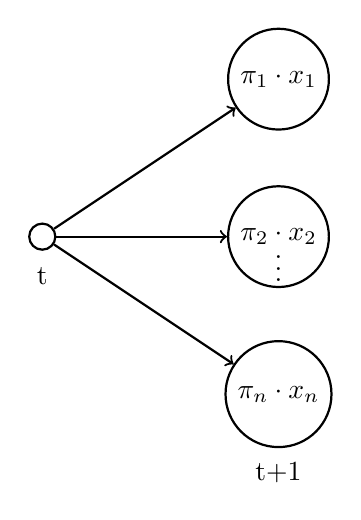
\begin{tikzpicture}[->, thick, auto, node distance=3cm]
    % Nodes at t
    \node[circle, draw] (t) at (0, 0) {};
    
    % Nodes at t+1
    \node[circle, draw] (t1s1) at (3, 2) {\(\pi_1 \cdot x_1\)};
    \node[circle, draw] (t1s2) at (3, 0) {\(\pi_2 \cdot x_2\)};
    \node[circle, draw] (t1sn) at (3, -2) {\(\pi_n \cdot x_n\)};

    % Edges
    \draw (t) -- (t1s1);
    \draw (t) -- (t1s2);
    \draw (t) -- (t1sn);
    
    % Labels for time
    \node at (0, -0.5) {t};
    \node at (3, -3) {t+1};
    
    % Dots for multiple nodes
    \node at (3, -0.3) {\(\vdots\)};
\end{tikzpicture}
    \caption{States of the world at time \(t+1\)}
    \label{fig:states_of_the_world}
\end{figure}

\section{Utility and Asset Pricing}

We want to find the value of the payoff $x_{t+1}$ at time $t$ to an 
investor. We describe the investor's preferences using an 
\textit{utility function}:

\begin{equation}
    U(c_t, c_{t+1}) = u(c_t) + \beta u(c_{t+1})
\end{equation}

where $c_t$ is consumption at time $t$, $c_{t+1}$ is consumption at
time $t+1$, $u(c_t)$ is the utility of consumption at time $t$.
$\beta$ is the \textit{discount factor} that measures how much the
investor values consumption at time $t+1$ relative to consumption at
time $t$. 

The point of the utility function is to capture the investor's
aversion to \textit{risk} and \textit{delay}, and 
discounting prices accordingly. 
Asset pricing depends on what are people willing to pay for.
It depends on how impatient and risk averse they are.
An example is the logarithmic utility function. In that case,
if $u(c) = \log(c)$, then $u'(c) = 1/c$. 

$u(c)$ is the level of utility from consumption. It can be described 
as the level of happiness of the investor. $u'(c)$ is the 
marginal utility of consumption. It can be roughly described as 
hunger of the investor.
If $u'(c) > 0$ when $u(c)$ rises, it means that people 
always want more consumption. If $u'(c) < 0$ when $u(c)$ rises,
then $u(c)$ is concave, and hunger decrease as you eat more.
$\beta$ is a number, typically 0.95. People prefer money now 
than later, they dislike delay. $\beta$ captures their impatience.
$c_{t+1}$ is random. You don't know at time $t$ how things will 
turn out, what $c_{t+1}$ will be.

\begin{tcolorbox}[colback=white, colframe=black, title=Example X]
    xxx
\end{tcolorbox}

A more useful utility function is the \textit{power utility function}:

\begin{equation}
    u(c) = \frac{c^{1-\gamma}}{1-\gamma}
\end{equation}

In that case, $u'(c) = c^{-\gamma}$, and $\gamma$ is the \textit{risk aversion} parameter.
If $\gamma = 1$, then $u(c) = \log(c)$ and 
$u'(c) = 1/c$. 

This functional form lets you have more or less curved function,
that is more or less risk aversion.

\begin{tcolorbox}[colback=white, colframe=black, title=Example X]
    power utility function and marginal utility function
\end{tcolorbox}

\section{Risk Valuation}

To apply what we have learned so far to risk valuation, we can start
from the definition of the covariance:

\begin{equation}
    \text{Cov}(m, x) = E(mx) - E(m)E(x)
\end{equation}

Thus,

\begin{equation}
    p = E(mx) = \text{Cov}(m, x) + E(m)E(x)
\end{equation}

\begin{equation}
    p = \frac{1}{R^f} E(x) + \text{Cov}(m, x)
\end{equation}

with the approximation

\begin{equation}
    m_{t+1} \approx 1 - \delta - \gamma \Delta c_{t+1}
\end{equation}

we have

\begin{equation}
p^i_t \approx \frac{1}{R^f} E(x^i_{t+1}) + \text{Cov}(x^i_{t+1}, \Delta c_{t+1})
\end{equation}

That is, the price is lower if the asset do well 
when consumption is low, and vice versa. Prices are higher 
for assets that provide insurance against consumption risks.
Prices are low for assets that, if you buy them, make your consumption
more risky. 

In risk valuation, the covariance term really matters. 
The same $m$ and the same $x$ can have different prices depending on the covariance between
$m$ and $x$. 

\begin{tcolorbox}[colback=white, colframe=black, title=Example 1]
Suppose there are two states $u$ and $d$ tomorrow, with probability
$1/2$ each. In state $u$, consumption is high, and in state $d$,
consumption is low.

\begin{equation}
    p_t = E(m, x) = \frac{1}{2} m_u x_u + \frac{1}{2} m_d x_d
\end{equation}


Suppose $x$ pays off well in good times if $x_u = 2$ and 
$x_d = 1$. Suppose also that $m_u = 0.5$ and $m_d = 1$. 
Then,

\begin{equation}
    p_t = \frac{1}{2} \times 0.5 \times 2 + \frac{1}{2} \times 1 \times 1 = 1
\end{equation}

Now suppose we keep the same volatility but $x$ pays off well 
in bad times and badly in good times, with $x_u = 1$ and $x_d = 2$.

Then,

\begin{equation}
    p_t = \frac{1}{2} \times 0.5 \times 1 + \frac{1}{2} \times 1 \times 2 = 1.25
\end{equation}

The payoff is worth more in the second case because it pays off
more in bad times, that is when $m$ is high (hungry) rather 
than $m$ is low (full). 
$m$ acts like a price: it says that payoffs 
delivered in the bad state of nature $d$ worth more than 
payoffs delivered in the good state of nature $u$.

\end{tcolorbox}

In the previous part, we had the discount factor of the form:

\begin{equation}
    p^i_t = \frac{E(x^i_{t+1})}{ER^i}
\end{equation}

where $ER^i$ is the expected return on the asset.
Our new version is:

\begin{equation}
    p^i_t = E(m_{t+1}x^i_{t+1})
\end{equation}

where $m_{t+1}$ is the stochastic discount factor. It is 
stochastic in the sense that it is unknown at time $t$, 
and therefore is inside the expectation. It is the same 
for all assets. Different covariance of 
$m_{t+1}$ with $x^i_{t+1}$ gives different risk adjustments
for different assets.

\section{Risk and Beta}

In this section, we will see that $p = E(mx)$ implies:

\begin{equation}
E(R^{ei}) = -R^f \text{Cov}(R^{ei}, m) = \beta_{R^{ei},m} \lambda_m
\end{equation}

where $\beta_{R^{ei},m}$ is the beta of the asset $i$ with respect to $m$.

\subsection{Expected Excess Returns and Covariance}

We start with the fact that if \textit{excess} returns or 
zero-cost portfolios have price 0, then, when excess returns 
$R^e = R^i - R^f$
is the payoff, $p = E(mx)$ implies:

\begin{equation}
    0 = E_t(m_{t+1}R^{e}_{t+1})
\end{equation}

Using again the definition of the covariance and looking 
to obtain the betas:

\begin{equation}
    \text{Cov}(m, x) = E(mx) - E(m)E(x)
\end{equation}

\begin{equation}
    E(mx) = \text{Cov}(m, x) + E(m)E(x)
\end{equation}

Then 

\begin{equation}
    0 = E(mR^e) = E(m)E(R^e) + \text{Cov}(m, R^e)
\end{equation}

\begin{equation}
    E(m)E(R^e) = -\text{Cov}(m, R^e)
\end{equation}

\begin{equation}
    E(R^e) = - R^f \text{Cov}(m, R^e)
\end{equation}

\subsection{Betas Formulation}

We can reformulate our previous result in terms of betas:

\begin{equation}
    E(R^e) = \frac{\text{Cov}(m, R^e)}{var(m)}[-R^f var(m)]
\end{equation}

\begin{equation}
    E(R^e) = \beta_{R^e, m} \lambda_m
\end{equation}

We can now link it directly to consumption. If $m_{t+1} = a - bf_{t+1}$
then:

\begin{equation}
    E(R^e) = -R^f \text{Cov}(R^e, m) = R^f \times b \times cov(R^e, f)
\end{equation}

\begin{equation}
    E(R^e) = \frac{\text{Cov}(R^e,f)}{var(f)}[R^f \times b \times var(f)] = \beta_{R^e,f} \lambda_f
\end{equation}

So, using $m_{t+1} \approx 1 - \delta - \gamma \Delta c_{t+1}$, we have:

\begin{equation}
    E(R^e) \approx -\text{Cov}(1 - \delta - \gamma \Delta c_{t+1}, R^e) \approx \gamma \text{Cov}(\Delta c_{t+1}, R^e)
\end{equation}

where we also have assumed that $R^f \approx 1$. We finally have:

\begin{equation}
    E(R^e) \approx \beta_{R^e, \Delta c} \times \lambda_c
\end{equation}

\subsection{Interpreting Excess Return and Beta Relationship}

In regression terms, it means that we can run time series 
regressions to find betas:

\begin{equation}
    R^i_{t+1} = \alpha_i + \beta_{i,\Delta c} \Delta c_{t+1} + \epsilon^i_{t+1}
\end{equation}

The average returns should indeed be linearly related to 
betas:

\begin{equation}
    E(R^i) = R^f + \beta_{i,\Delta c} \lambda_c
\end{equation}

where $\beta$ is the right hand variable (the usual $x$) and 
$\lambda$ is the slope (usually the $\beta$).

\begin{figure}[htbp]
    \centering
\begin{tikzpicture}
    % Axis
    \draw[<->] (0, 5) node[above] {$E(R^i)$} -- (0, 0) -- (5, 0) node[right] {\(\beta_i\)};
    
    % Line
    \draw[thick, blue] (0, 0) -- (4, 4) node[above] {slope \(\lambda\)};
    
    % Labels
    \node[below left] at (0, 0) {0};
    \node[below right] at (2, 2) { $E(R^i) = \lambda \beta_i$};
    \node[below] at (4, 0) {1};
    \node[left] at (0, 4) {1};
\end{tikzpicture}
    \caption{Expected Return and Beta Relationship}
    \label{fig:expected_return_beta}
\end{figure}

The superscript $i$ emphasizes that this is about 
why average returns of one asset are higher than of another 
(cross section). This is not about the fluctuation in ex-post return
or predicting returns. $E(R^i)$ is the reward, $\beta_i$ the 
quantity of risk that varies across assets $i$, and 
$\lambda$ is the price of risk (it is common to all assets).

An asset must offer high $E(R^i)$ (reward) to compensate
the investors for high $\beta_i$ (risk). 
Assets that covary negatively with $m$, hence positively 
with consumption growth, must pay a higher average return. 


\begin{tcolorbox}[colback=white, colframe=black, title=Example X]
    


\end{tcolorbox}


\begin{figure}[htbp]
    \centering
    \begin{tikzpicture}
        % Draw the axes
        \draw[<->] (0, 5) node[above] {\(p\)} -- (0, 0) -- (3, 0) node[right] {Time};
        
        % Draw the lines for the two assets
        \draw[thick, blue] (0.5, 1) -- (2.5, 4) node[near end, right, below] {};
        \draw[thick, red] (0.5, 3) -- (2.5, 3.5) node[midway, above] {};
        
        % Add points for Asset 1
        \node[below] at (0.5, 1) {\(p_1^t\)};
        \node[above] at (2.5, 4) {\(p_1^{t+1}\)};
        \draw[fill=blue] (0.5, 1) circle (2pt);
        \draw[fill=blue] (2.5, 4) circle (2pt);
        
        % Add points for Asset 2
        \node[below] at (0.5, 3) {};
        \node[above] at (2.5, 3.5) {};
        \draw[fill=red] (0.5, 3) circle (2pt);
        \draw[fill=red] (2.5, 3.5) circle (2pt);
        
        % Label the times
        \node[below] at (0.5, 0) {\(t\)};
        \node[below] at (2.5, 0) {\(t+1\)};
    \end{tikzpicture}
    \caption{High $E(R^i)$ = Low $p^i$}
    \label{fig:asset_pricing}
\end{figure}

Given a certain amount of volatility (price must move at some point),
price (risk-discount) depends on when good/bad performance occurs.
Average returns are high if beta on $m$ or $\Delta c$ is large.
Stocks must pay high returns if they tend to go down 
in bad times. Price is depressed if a payoff is low in 
bad times, when the investor is hungry (high $m$, low $\Delta c$), 
therefore we have high $E(R^i)$.
Price is high if a payoff is high in bad times, when the investor
is full (low $m$, high $\Delta c$). Therefore we have low $E(R^i)$.
Higher $\gamma$ (risk aversion) implies larger price effects.

The variance $\sigma(R^e)$ of an individual asset 
does not matter, only its covariance with $m$ (\textit{e.g.} consumption growth)
matters. Recall that we have the following:

\begin{equation}
    R^{ei} = \beta_{i,m} m + \epsilon^i 
\end{equation}

Therefore the variance is:
\begin{equation}
    var(R^{ei}) = \beta^2_{i,m} \sigma^2_{m} + \sigma_{\epsilon^i}^2
\end{equation}

and the second component of variance has no effect on mean returns.

\section{CAPM and Multifactor models}

We can relate what we have seen so far to the CAPM and Fama-French model. 
This underlines the economic rationale for $E(hml)$, $E(smb)$, and so forth.

To do so, we start from:

\begin{equation}
    E(R^{ei}) = R^f \text{Cov}(R^{ei}, m) = \beta_{R^{ei}, m} \lambda_m
\end{equation}

We find reasons to say:

\begin{equation}
    m = a -b \times f 
\end{equation}

to get 

\begin{equation}
    E(R^{ei}) = \beta_{R^{ei}, f} \lambda_f
\end{equation}

with the full algebra to be:

\begin{equation}
    E(R^{ei}) = R^f \text{Cov}(R^{ei}, f \times b) = R^f \text{Cov}(R^{ei}, f) \times b 
    = \frac{\text{Cov}(R^{ei}, f)}{var(f)} \times [R^f \times b \times var(f)] 
\end{equation}

The intuition is to say that if low $f$ indicates bad times, 
when people are hungry, then assets which pay off badly in times 
of low $f$ must have low prices and deliver high expected returns.




\section{Conclusion}

What we have seen here is the beginning of all asset pricing 
models. In the empirical version, we'll see that 
we use risk factors instead of $\Delta c$.